%%
%% This is file `mcmthesis-demo.tex',
%% generated with the docstrip utility.
%%
%% The original source files were:
%%
%% mcmthesis.dtx  (with options: `demo')
%% !Mode:: "TeX:UTF-8"
%% -----------------------------------
%%
%% This is a generated file.
%%
%% Copyright (C)
%%     2010 -- 2015 by latexstudio
%%     2014 -- 2016 by Liam Huang
%%     2014 -- 2016 by latexstudio.net
%%
%% This work may be distributed and/or modified under the
%% conditions of the LaTeX Project Public License, either version 1.3
%% of this license or (at your option) any later version.
%% The latest version of this license is in
%%   http://www.latex-project.org/lppl.txt
%% and version 1.3 or later is part of all distributions of LaTeX
%% version 2005/12/01 or later.
%%
%% This work has the LPPL maintenance status `maintained'.
%%
%% The Current Maintainer of this work is Liam Huang.
%%
\documentclass{mcmthesis}
\mcmsetup{CTeX = false,   % 使用 CTeX 套装时,设置为 true
        tcn = 2010755, problem = A,% 队伍控制号码,接受一个字符串作为值;选题,接受一个字符串作为值;
        sheet = false, %为真时将输出摘要页,否则不输出;默认为 true。
        color = red,  %设置控制页的题目号的颜色
        titleinsheet = true, %为真时将在摘要页输出标题,否则不输出;默认为 false。
        keywordsinsheet = true,%为真时将在摘要页输出关键字,否则不输出;默认为 false。
        titlepage = false,%为真时将输出标题页,否则不输出;默认为 true。
        abstract = true}%为真时将在标题页输出摘要和关键词,否则不输出;默认值为 true。
\usepackage{palatino}  %控制正文字体,若是不喜欢可以注释掉。
\usepackage{lipsum}
\usepackage{tikz}
\usepackage{xcolor}
\usepackage{verbatim}
\usepackage{subfigure} 
\usetikzlibrary{arrows,shapes,chains}
\title{Title!}
\author{\url{http://www.latexstudio.net}\\[3pt]  \href{http://www.latexstudio.net/}
  {\includegraphics[width=7cm]{mcmthesis-logo}}}
\date{\today}

\makeatletter
\renewcommand*\l@section{\@dottedtocline{1}{12pt}{12pt}}
\makeatother

%%%%%%%%%%%%%%%%%%%%%%%%%%%%%%%%%%%%%%%%
%% MCM/ICM LaTeX Template %%
%% 2020 MCM/ICM           %%
%%%%%%%%%%%%%%%%%%%%%%%%%%%%%%%%%%%%%%%%
\usepackage{geometry}
\geometry{left=1in,right=0.75in,top=1in,bottom=1in}

%%%%%%%%%%%%%%%%%%%%%%%%%%%%%%%%%%%%%%%%
% Replace ABCDEF in the next line with your chosen problem
% and replace 1111111 with your Team Control Number
\newcommand{\Problem}{A}
\newcommand{\Team}{\# 2010755}
%%%%%%%%%%%%%%%%%%%%%%%%%%%%%%%%%%%%%%%%

\usepackage{newtxtext}
\usepackage{amsmath,amssymb,amsthm}
\usepackage{newtxmath} % must come after amsXXX

%\usepackage[pdftex]{graphicx}

\usepackage{fancyhdr}
\lhead{Team \Team}
\rhead{}
\cfoot{}

\newtheorem{theorem}{Theorem}
\newtheorem{corollary}[theorem]{Corollary}
\newtheorem{lemma}[theorem]{Lemma}
\newtheorem{definition}{Definition}

%%%%%%%%%%%%%%%%%%%%%%%%%%%%%%%%
\begin{document}
\graphicspath{{.}}  % Place your graphic files in the same directory as your main document
\DeclareGraphicsExtensions{.pdf, .jpg, .tif, .png}
\thispagestyle{empty}
\vspace*{-16ex}
\centerline{\begin{tabular}{*3{c}}
	\parbox[t]{0.3\linewidth}{\begin{center}\textbf{Problem Chosen}\\ \Large \textcolor{red}{\Problem}\end{center}}
	& \parbox[t]{0.3\linewidth}{\begin{center}\textbf{2020\\ MCM/ICM\\ Summary Sheet}\end{center}}
	& \parbox[t]{0.3\linewidth}{\begin{center}\textbf{Team Control Number}\\ \Large \textcolor{red}{\Team}\end{center}}	\\
	\hline
\end{tabular}}
\begin{Huge}
\begin{center}
\textbf{Escape From Scotland}
\end{center}
\end{Huge}
%%%%%%%%%%% Begin Summary %%%%%%%%%%%
% Enter your summary here replacing the (red) text
% Replace the text from here ...
\begin{center}
\begin{large}
\textbf{Summary}
\end{large}
\end{center}

Firstly, based on the data in the ICES working document\cite{3}\cite{4},we use \textbf{Generalized Additivity Model (GAM)} to analyze the relationship between fish density and environmental factors. By utilizing the results of Generalized Additive Model ,we get the environmental fitness formula of fish. Then we use this formula to calculate the situation in 30 different sea areas,and finally we use \textbf{Continuous-time Markov Model} to calculate the situation in each area in the next 50 years. From the rectangle state, we can infer the living area of mackerel and herring.\\

Secondly, in order to figure out the affection on the fish’s occurrence position caused by temperature, we collect the temperature data of North Sea from 2009 to 2019. Then we divide the ocean into grids by longitude and altitude. After analyzing we find that the change of the temperature is highly relevant with season, which tends to increase. We establish a \textbf{Seasonal Autoregressive Integrated Moving Average Model (SARIMA)} to predict the temperature change in the next 50 years. Next, we represent the position of the fish population by finding the clustering center. We use \textbf{Mean-Shift Algorithm} to get cluster centers of each years and look up the surrounding temperature. Then we build a liner regression to find out the relationship between year and fish's favorite temperature. After that we construct a \textbf{Score Function} to determine whether a region will become a cluster center in the future or not. The main idea of the function is to predict the temperature of one region and its surroundings. The higher score a region gets,the higher possibility it will be chosen by fish.\\

Thirdly, to provide constructive suggestions for fishing companies in Scotland, we build a \textbf{Similarity to an Ideal Solution (TOPSIS)} to evaluate the several strategies. We consider different factors such as the maintenance of facilities, the cost of relocation and fuel, the total catch of each strategy. We use \textbf{Analytic Hierarchy Process (AHP)} to determine the weight of each factor, then sort strategies in ascending order by calculating the distance from each strategy to the optimal one. In this way, we conclude that relocation is a reasonable and sustainable choice in the long term.\\


Next, considering the fact that territory seas of countries restricts the effective fishing, we collect data from the United Nations Convention on the Law of the Sea (LOSC). By calculating the frequency of fish appearance in available seas we calculate the quantity of total catch. Then we define the \textbf{loss rate} to describe the impact of territorial limits and get the conclusion that as mackerel and herring migrating to the north, the loss of fishing companies grow larger.\\

Besides the models we established, we complete the Sensitivity Analysis and prove the stability of our models. Finally, we write an article on the basis of results we get to help fishermen.\\


\textbf{Keywords}: \textbf{Generalized Additive Model (GMA)}, \textbf{Continuous-time Markov Model}, \textbf{Seasonal Autoregressive Integrated Moving Average Model( SARIMA Model)}, \textbf{Mean-Shift Algorithm}, \textbf{Similarity to an Ideal Solution (TOPSIS)}

% to here
%%%%%%%%%%% End Summary %%%%%%%%%%%

%%%%%%%%%%%%%%%%%%%%%%%%%%%%%%
\clearpage
\pagestyle{fancy}

% Uncomment the next line to generate a Table of Contents
%\tableofcontents 

\setcounter{page}{1}
\rhead{Page \thepage\ of \pageref{LastPage}}
%%%%%%%%%%%%%%%%%%%%%%%%%%%%%%


\begin{abstract}
Firstly,\cite{1}

Secondly,

Thirdly,

We then

Finally,

\begin{keywords}
Generalized Additive Model, Markov model
\end{keywords}
\end{abstract}
\maketitle

\tableofcontents


\section{Introduction}
\subsection{Restatement of the Problem}

We need to build mathematical models to solve following problems:

\begin{enumerate}
\item From a number of perspectives, our mathematical model needs to determine where mackerel and herring are most likely to appear in the next 50 years, with temporal and spatial environmental factors considered.
\item Our second task is to establish two model, one of them is the ocean temperature prediction model, the other one is fish occur position prediction model.
\item Strategies require to be determined to help small companies.
\end{enumerate}


\subsection{Overview of Our Work}
We searched a large number of papers that discuss the condition of herring and mackerel to help us deepen the understanding of the problem.

Firstly,based on the data in the ICES working document\cite{3}\cite{4}, we establish a \textbf{Generalized Additive Model }(GAM) to analyze the relationship between fish stocks and environmental impact factors.Then we find out the key factors that influenced the model and select the optimal spatial distribution prediction model to provide scientific basis for predicting the spatial distribution of herring and mackerel.We get the environmental fitness formula of fish. Then we used the formula to calculate the situation in 30 different sea areas, and finally we use \textbf{Continuous-time Markov model} to calculate the situation in each area in the next 50 years. From the rectangle state, we  predict the mackerel’s living area and herring’s living area.\\

For the second question, firstly we choose North Sea as our target to implement temperature prediction. Considering the pattern of temperature change is highly relevant with season, we establish a Seasonal Autoregressive Integrated Moving Average Model to predict the temperature of North Sea in the next 50 years base on the temperature date from Hadley Centre observations office. Then we decide to use cluster center point to represent the distribution of fish and calculate the position of cluster centers by Shift Means algorithm   base on the data from ICES. Finally we build a model to predict the occur position(cluster center) of fish in the future by analyzing the relationship between year and the temperature around the cluster center and combining the result of temperature prediction. We conclude that in the worst case, small fishery companies will get into trouble for the extra voyage distance after 2025 and the best case is after 2045.\\


\section{Assumption}
To simplify our model, we make following well-justified assumptions.
\begin{enumerate}[(1)]
\item Carbon emissions will increase at a certain rate as well as sea surface temperature in the next 50 years.
\item  Effect of the weather is neglected.
\item Sea temperature can be represented by the sea surface temperature in this region.
%
\item	Fishing operation is always carried out on July or August.
\item We divided the selected rectangular sea area $(44^\circ N20^\circ W\sim68^\circ N30^\circ E) $ equally into 30 equal parts.In order to simplify the calculation, it is assumed that the fish are evenly distributed in each rectangular area (the longitude span is 10$^\circ$ and the latitude span is 4$^\circ$) with the same environmental and spatial factor.
%
\item The population density of species remain relatively constant during a year.
\item The quantity of mackerel and herring is in proportion to their frequency of occurrence.
~\\~\\~\\~\\~\\~\\~\\~\\~\\~\\~\\
\end{enumerate}
\subsection{Symbols and Definition}
There are some symbols appear in the model. We show them below:
\begin{table}[htbp]
\centering
\caption{Symbols in Chapter 3}
\begin{tabular}{cp{0.8\textwidth}}
\toprule
 Symbols & Description\\
\midrule
 $i$ & Station variable \\
 $DS_i$ & Density of fish( mackerel or herring) at station i $(kg/km^2)$\\
 $H_i$ & Horizontal opening of trawl at station i  $(km)$\\
 $TD_i$ & Distance of the trawl haul $(km^2)$ \\
 $C_i$ &  Catch at station i$(kg)$\\

  $\lambda_i$ &   Longitude at station i $(^\circ W)$\\
 $\phi_i$ &   Latitude at station i $(^\circ N)$\\
$SST_i$ &  Sea Surface Temperature at station i $(^\circ C)$\\

 $z_i$ & Zooplankton's dry weight at station i $(kg)$\\
 $SSB_i$ &  Spawning-stock biomass at station i \\
  $b_i$ & Number of biological species at station i\\
$y$ & Year \\
$j$& Rectangular number\\
$t$ & Time  \\
$M_j(t)$ & State of the $j_{th}$ rectangle at time $t$ \\
$P_{M_w,M_k}$ &  Transition probability for the State $M_w$changing into State $M_k$\\
\bottomrule
\end{tabular}
\end{table}
\begin{table}[htbp]
\centering
\caption{Symbols in Chapter 4}
\begin{tabular}{cp{0.8\textwidth}}
\toprule
 Symbols & Description\\
\midrule
$B$ &  Backshift operator\\
$x_{t}$ & Temperature of a region of seawater in $t_{th}$ month.\\
$P, Q$ & Orders\\
$T_{b}$ & Average temperature\\
$R_{s}$  & Coastal region\\
$R_{t}$ & Inland region \\
$r(lo,la)$ & Temperature of a region with geographical coordinates ($lo$, $la$)\\
\bottomrule
\end{tabular}
\end{table}
\begin{table}[htbp]
\centering
\caption{Symbols in Chapter 5 \& 6}
\begin{tabular}{cp{0.8\textwidth}}
\toprule
 Symbols & Description\\
\midrule
 %\rowcolor{lightgray}
$CPUE_{y}$ & Catch Per Unit Effort in year $y$\\
$F$  & Funds\\
$M$  & Maintenance cost\\
$T$  & Transportation fee\\ 
$s_{j}$  & Area of $j_{th}$ square\\
$A $  & Comparison matrix\\
$W$ & Weight\\
$y$ & Year\\
$L_{y}$ & Quantity of fish in the year $y$\\
$C$ &  Appearance of mackerel\\  
\bottomrule
\end{tabular}
\end{table}





\section{Migration Model of Mackerel and Herring}
We first establish a Generalized Additive Model(GAM) to predict the relationship between fish density changes and spatiotemporal factors.Then,we use the Continuous-time Markov model to calculate the state of each rectangular sea area in
the next 50 years. From the rectangle state, we can infer the mackerels living area
and herrings living area.In the figure below,Z stands for  zooplanktons dry weight, B stands for the number of biological species.
\begin{figure}[htbp]
\centering
\tikzstyle{format}=[circle,draw,aspect=5,fill=blue!10,text width=1.6cm,text centered,font=\sffamily,scale=1]
\tikzstyle{test}=[font=\sffamily,rectangle,aspect=5,fill=blue!25,draw,thin,scale=1]
\tikzstyle{t}=[circle,aspect=5,fill=blue!30,draw,thin]
		\tikzstyle{point}=[coordinate,on grid,]
		\begin{tikzpicture}[->,>=stealth',shorten >=1pt,auto,node distance=2.3cm,
    thick,base node/.style={circle,draw,minimum size=20pt}, real node/.style={double,circle,draw,minimum size=35pt}]
            \node[format](n){Year};
			\node[format,right of = n] (n0){Longitude};
			\node[format,right of=n0] (n1){Latitude};
			\node[format,right of=n1] (n2){SST};
			\node[format,right of=n2] (n3){SSB};
            \node[format,right of=n3] (n4){Z};
			\node[format,right of=n4] (n5){B};

            \node[test](n21)at(0,-2.5){Time factor};
            \node[test](n22)at(3.8,-2.5){Spatial factors };
            \node[test](n23)at(10.8,-2.5){Environmental factors };

            \node[test,fill=blue!40](n31)at(6,-4){The most likely locations for mackerel and herring to live over next 50 years};
            			
			\draw[->] (n) -- (n21);
\draw[->] (n0) -- (n22);
\draw[->] (n1) -- (n22);
\draw[->] (n2) -- (n23);
\draw[->] (n3) -- (n23);
\draw[->] (n4) -- (n23);
\draw[->] (n5) -- (n23);
\draw[->,dashed] (n21) -- (n31);
\draw[->,dashed] (n22) -- (n31);
\draw[->,dashed] (n23) -- (n31);	
		\end{tikzpicture}
        \caption{Parametric analysis of the model.}
\end{figure}



\subsection{Prediction of Fish Migration based on Generalized Additive Model}
\textbf{The Generalized Additive Model} (GAM), which is flexible and focuses more on the complex relationship between detection data, has been widely used in the fishery field.
\subsubsection{Construction of GAM}
At each station, Mackerel density per station $(DS; kg/km^2) $ is calculated as:
\begin{equation}
DS_i=\frac{C_i}{TD_i*H_i}
\end{equation}

Thanks to ICES Working Group for the data\cite{1}\cite{4}. We get the horizontal opening of the trawl $H_i$, the distance towed by the trawl $TD_i$ and the mackerel catch $C_i$ used in calculations.
The model expression of\textbf{ GAM} is as follows:

\begin{equation}
In DS_{i,(\lambda,\phi)} = a + s1(\lambda_i,\phi_i) + s2(SST_i) + s3(b_i) +s4(z_i)+ s5(y)+\beta*SSB_i + \varepsilon
\end{equation}

where $In DS_{i,(\lambda,\phi)}$ is a link function, $a$  is the model intercept, $\lambda_i$ is longitude at station i, $\phi_i$ is latitude, $SST_i$ is Sea Surface Temperature ,$b_i$ is the number of biological species , $z_i$ is zooplankton’s dry weight , $SSB_i$ is the estimated mackerel spawning stock biomass with linear coefficient $\beta$, s1 is a two-dimensional smoothing function, $y$ is year, $s2\thicksim s5$ are one dimensional smoothing functions for temperature and mesozooplankton, and $\varepsilon$ is the error term.




\subsubsection{Optimization of GAM}
We select variables with significant influence on $DS_i$.The GAM model is used to test the significance of environment factors and annual resources of mackerel population, so as to obtain statistically significant influence factors.

\begin{table}[htbp]
\centering
\caption{ Test of GAM between the Environmental or Climatic Factors.}
\begin{tabular}{ccc}
 \hline
 \rowcolor{lightgray}\makebox[0.3\textwidth][c]{Factor}& \makebox[0.3\textwidth][c]{p-value}& \makebox[0.3\textwidth][c]{$R^2$}\\ \hline
 SST	& $0.0275^*$&0.677\\[3pt]
latitude	    & $0.0134^*$&0.606\\[3pt]
 longitude         & $0.0795^.$&0.329\\[3pt]
 y	& $0.00338^{**}$&0.76\\[3pt]
  B	& $0.0222^*$&0.541\\[3pt]
Z & $0.0163^*$&0.705\\[3pt]\hline
\end{tabular}\\

 \textbf{Note: ** indicates a significant correlation at a significance level of only $\alpha$=0.05 (bilateral).}
\end{table}

According to the comprehensive analysis of expert knowledge\cite{2} , SST, SSB,latitude, longitude were retained in the model.
The  expression of optimized GAM is as follows:
\begin{equation}
In DS_{i,(\lambda,\phi)} = a + s_1(SST_i)+s_2(y)+s_3(z_i)+\beta*SSB_i + \varepsilon
\end{equation}



\subsubsection{Results of GAM model}
 Result is obtained by using the “mgcv” package in R 3.6.2. The following figure shows the relationship diagram of the mackerel density of each factor calculated by GAM. $W$ stands for longitude, $N$ stands for latitude.
  \begin{figure}[htbp]
\small\centering
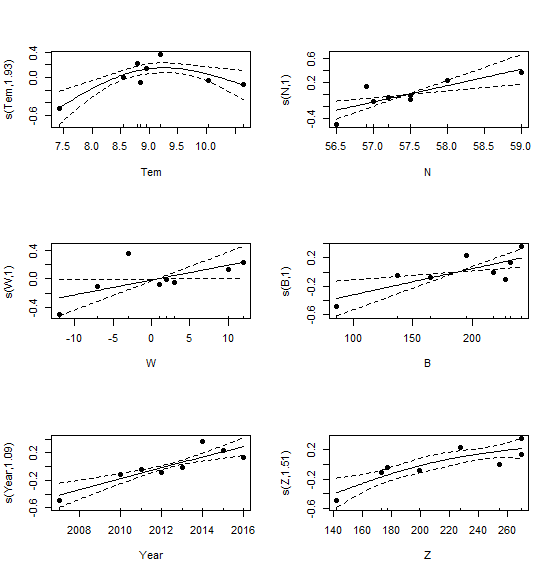
\includegraphics[width=7cm]{./figures/presult.png}
\caption{The relationship between factors and the density of mackerel}
\end{figure}
\begin{itemize}
\item \textbf{Steric factor : }
It can be seen from the spatial factors that mackerel is concentrated in latitude $56.5^\circ N\sim 58.5^\circ N$, longitude $-7^\circ W\sim 10^\circ W$. Figure 2 shows the tendency of mackerel to migrate northward.In terms of longitude, Mackerel shoals tend to migrate eastward (toward the Norwegian sea) and westward (toward Greenland).
\item \textbf{Environmental factor : }The results of GAM model shows that SST is the most important habitat indicator affecting mackerel migration. When the temperature is between 8$^\circ C$ and 10$^\circ C$ , the effect of temperature on fish density increases with the increase of temperature.The greater the plankton biomass in the middle layer, the larger the fish population.It also shows that the greater the number of species, the greater the number of fish.
\end{itemize}

\subsection{Future Location Prediction based on Continuous-time Markov Chain}
\subsubsection{Construction Continuous-time Markov Model}
We divide the selected rectangular sea area $(44^\circ N20^\circ W\sim68^\circ N30^\circ E) $ equally into 30 equal parts.Each part has a longitude span of 10 degrees and a latitude span of 4 degrees.
The results of the GAM model show that B and Z are positive indicators of fish's environmental fitness, and  SST is an interval indicator.
Hence, the environmental fitness formula of fish was obtained.
\begin{equation}
L_j(t)=\frac{b_j}{max\{b\}}+
\frac{z_j}{max\{z\}}+
\begin{cases}
1-\frac{d-SST_j}{d-d^*}& \text{$SST_j < d$}\\
1  &\text{$d\leq SST_j\leq e$}\\
1-\frac{SST_j-e}{e^*-e}  &\text{$SST_j > e$}
\end{cases}
\end{equation}

where $L_j(t)\in [0,3]$ stands for the degree to which each square is suitable for fish to live, $[d,e]$ stands for the optimal stability interval of SST($8^\circ C\sim10^\circ C$),$[d^*,e^*]$ stands for maximum tolerance interval($0^\circ C\sim25^\circ C$).\cite{1}
Since $L_j(t)$ can be considered as a function of time $t$, we use Continuous-time Markov chain to simulate the distribution change of mackerel.The condition of each rectangle is closely related to the population density of mackerel.To simplify the problem, we set the following 5 states by calculating the value of $L_j(t)$.

\begin{table}[htbp]
\centering
\caption{States of each rectangle}
\begin{tabular}{cp{0.8\textwidth}}
\toprule
 States & Meaning\\
\midrule
$M_{1}$ & most unsuitable for mackerel to survive \textbf{$(0\leqslant L_j<0.6)$}
$M_{1}$ = 1\\ \hline
$M_{2}$ & not suitable for mackerel to survive $(0.6\leqslant L_j<1.2)$
$M_{2}$ = 2\\ \hline
$M_{3}$&  suitable for mackerel to survive $(1.2\leqslant L_j<1.8)$
$M_{3}$ = 3\\ \hline
$M_{4}$& quite suitable for mackerel to survive $(1.8\leqslant L_j<2.4)$
$M_{4}$ = 4\\ \hline
$M_{5}$& most suitable for mackerel to survive$(2.4\leqslant L_j\leqslant 3.0)$
$M_{5}$ = 5\\
\bottomrule
\end{tabular}
\end{table}


Define $M_{j}(t)$ as the state of the $j_{th}$ rectangle at time $t$, $P_{wk}$ as the transition probability for the state $M_w$ changing into state $M_k$.  $M_w,M_k \in \{1,2,3,4,5\}$.\\
In random process$\{X(t),t\}$, for n=0,1,2..., in continuous time$t_0<t_1<...<t_b<...<t_{n+1}$, the following mathematical formula holds:

\begin{equation}
p(M_{wk})=p(M_w|M_k)=p_{M_{w}M_{k}}
\end{equation}
For any time $t\geq t_b$, the transfer probability can be written as:
\begin{equation}
p_{M_{w}M_{k}}(t_b,t)=P(M(t)=k|M(t_b)=w)
\end{equation}
Then we can get the Transition probability matrix $P$:
\begin{equation}
P =
\begin{bmatrix}
p_{11}     & \cdots & p_{15}      \\
\vdots & \ddots & \vdots \\
p_{51}      & \cdots & p_{55}
\end{bmatrix}
\end{equation}

Markov state transitin equation can be represented as:
\begin{equation}Q_{2} = Q_{1} P \end{equation}
\begin{equation} Q_{2}=
\begin{bmatrix}
M_{1}(0)      & \cdots & M_{5}(0)      \\
\vdots & \ddots & \vdots \\
M_{1}(t-1)     & \cdots &M_{5}(t-1)
\end{bmatrix}_{t\times5}
\end{equation}

\begin{equation}Q_{1}=
\begin{bmatrix}
M_{1}(1)      & \cdots & M_{5}(1)      \\
\vdots & \ddots & \vdots \\
M_{1}(t)     & \cdots &M_{5}(t)
\end{bmatrix}_{t\times5}
\end{equation}

According to least square method, we can get
\begin{equation}
P = (Q_{1}^TQ_{1})^{-1}Q_{1}^T Q_{2}
\end{equation}
Consequently, we can predict the state $M$ of each rectangle in the next 50 years.
\begin{equation}
Q_{50}=Q_1P^{50}
\end{equation}


\subsubsection{Results of Continuous-time Markov Model}
Since $M_5$ represents the state most suitable for mackerel survival, the smart fish will live in this area intensively.From the rectangle state, we can predict the mackerel's living area and herring's living area. Figure 3 shows the results.
\begin{figure}[htbp]
\small\centering
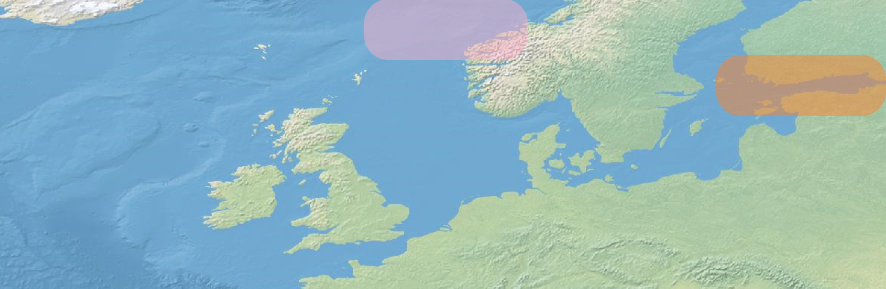
\includegraphics[width=11cm]{./figures/G2.png}
\caption{Population growth}
\end{figure}

The orange rectangle shows that the most likely place for herring to migrate is in \textbf{ Gulf of Bothnia}.
The pink rectangle shows where the mackerel is most likely to migrate is in \textbf{Norwegian Sea}.
The results of GAM shows that SST is the most important habitat indicator affecting fish migration.


\section{Time to Give a Warning}
\subsection{Temperature Prediction of Ocean}
\subsubsection{Introduction}
The temperature of Ocean is hard to predict because it is affected by many factors, mainly are sun radiation and marine atmospheric heat exchange and the ocean current make an obvious affection on local seawater. However, we can still find that the change of temperature is highly linked to the season change which means we can predict the temperature by using the former data. As a sequence of that, we decide to build SARIMA model as our solution.


\subsubsection{Prediction Model}
Due to hypotheses, the temperature of seawater is influenced by autocorrelation in time series and highly related to the season. As a consequence, we choose Seasonal ARIMA (SARIMA) Model \cite{1} to fit the curve. The general form of seasonal model SARIMA(p, d, q)(P, D, Q) is given by:
\begin{equation}
\Phi_{p}(B^s)\varphi(B)\nabla_{s}^{D}\nabla^{d} x_{t} = 
\Theta_{Q}(B^s)\theta(B)w_{t}
\end{equation} 

where $\{w_{t}\}$ is the nonstationary time series, usually is the usual Gaussian White noise process. $s$ is the period of the time series, here represent the month after 2019-12. The ordinary autoregressive and moving average components are represented by polynomials $\varphi(B)$ and $\theta(B)$ of orders $p$ and $q$. The seasonal autoregressive and moving average components are $\Phi_{p}(B^s)$ and $\Theta_{Q}B^{s}$, where $P$ and $Q$ are their orders.$\nabla^{d}$ and $\nabla_{s}^{D}$  are ordinary and seasonal difference components. $B$ is the backshift operator. The expressions are shown as follows:
\begin{equation} \varphi(B)=1-\varphi_{1}B - \varphi_{2}B^2 - \cdots- \varphi_{p}B^p \end{equation} 
\begin{equation} \Phi_{p}(B^s)=1-\varphi_{1}B^s - \varphi_{2}B^{2s} - \cdots- \varphi_{p}B^{ps}\end{equation}
\begin{equation} \theta(B)=1+\Theta_{1}B^s + \Theta_{2}B^{2s}+\cdots+\Theta_{Q}B^{Qs}\end{equation}
\begin{equation} \nabla^d = (1-B)^d \end{equation}
\begin{equation} \nabla_{s}^D=(1-B^s)^D\end{equation}
\begin{equation} B^k x_{t}=x_{t-k}\end{equation}
 $x_{t}$ represent the temperature of a region of seawater in $t_{th}$ month.\\
Firstly, we collect the time-series data of all regions. Here we choose 10 position and their analyze of temperature will write in the essay (appendix). In this character we will only show three of them (circle by red):
\textbf{}
\begin{figure}[h]
\centering
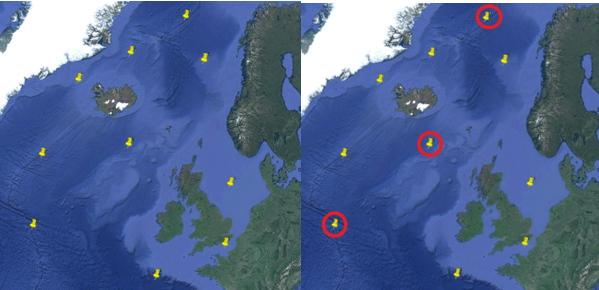
\includegraphics[width=7.5cm]{./figures/circle.png}
\caption{Position to Analyze}
\end{figure}
Time series analysis requires that the series should be stationarity. The basic idea of stationarity is that the probability laws that govern the behavior of the process do not change over time. If it’s not stationarity, then we should smooth it by using by using the difference equation. The result of  the chosen place is shown below:

\begin{figure}[htbp]
\centering
\subfigure[different equation result]{
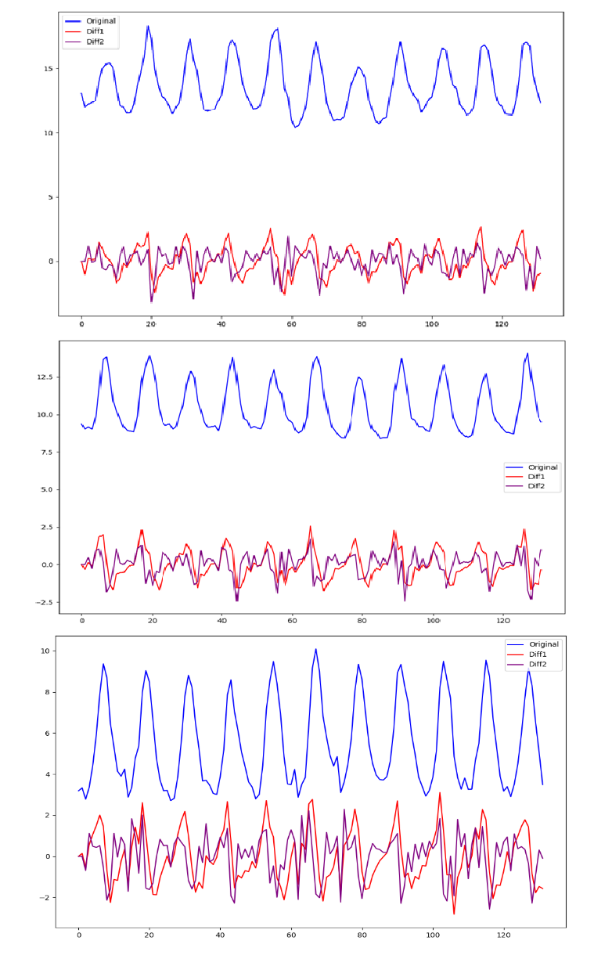
\includegraphics[width=4.5cm]{./figures/curve1.png}
%\caption{fig1}
}
\quad
\subfigure[ACF and PACF Result]{
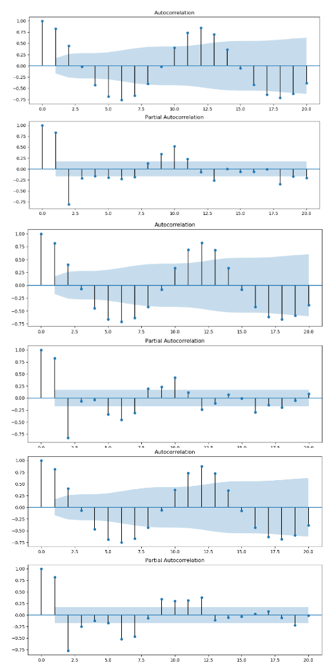
\includegraphics[width=3.7cm]{./figures/curve2.png}
}
\caption{Results}
\end{figure}
From the Autocorrelation Function (ADF) result and the different equation result above shows that d = 1 is well enough. As for the Autocorrelation Coefficient Function (ACF) and Partial Autocorrelation Fnuction (PACF) , there is no obvious tailing or truncation was found in the diagrams of the sequences ACF and PACF, which indicates that for such sequences, it is not suitable to fit the SARIMA model. Here we will use the time series decomposition (STL) method, and then use the SARIMA model to fit the trend series and the residual series. Here we only take the second one to go on.
\textbf{}
\begin{figure}[h]
\centering
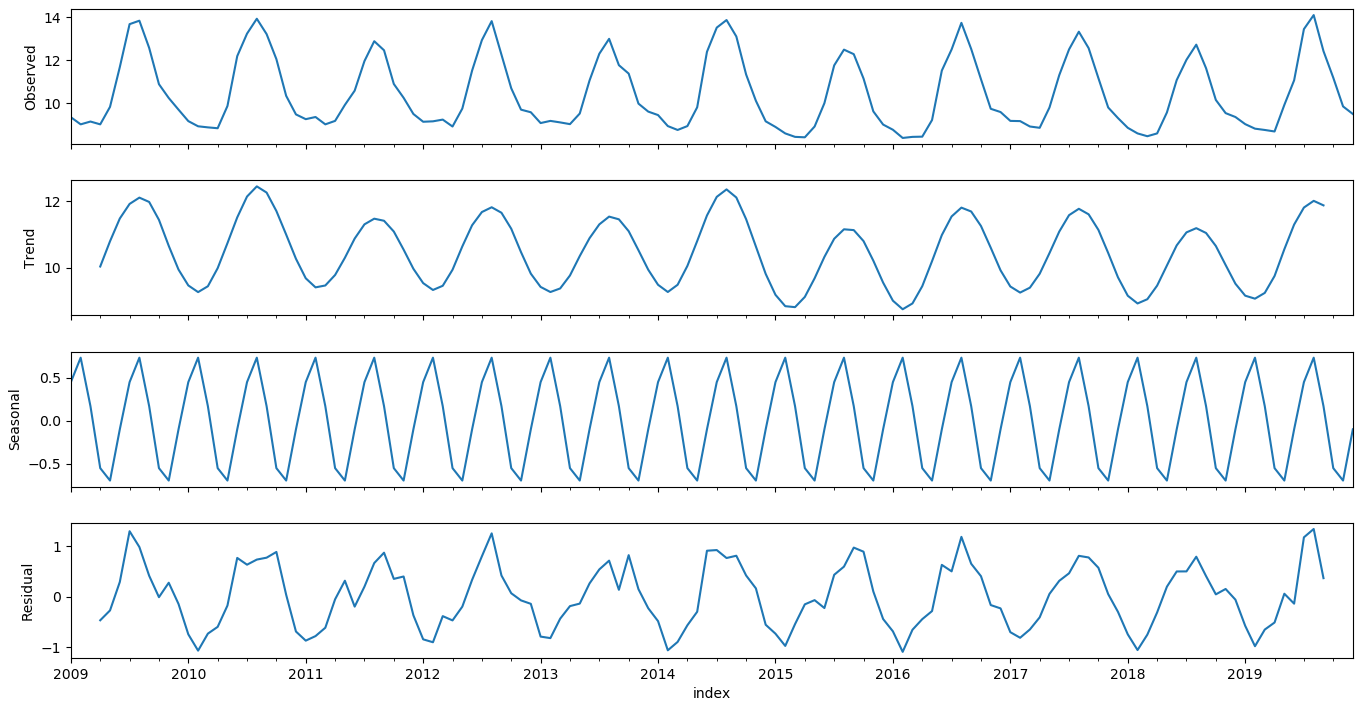
\includegraphics[width=4.5cm]{./figures/season.png}
\caption{STL Result}
\end{figure}
From the picture above, there is a certain periodic waving of seasonal. As a result, we decide to use SARIMA to fit the trend and residual.
\begin{figure}[htbp]
\centering
\subfigure[]{
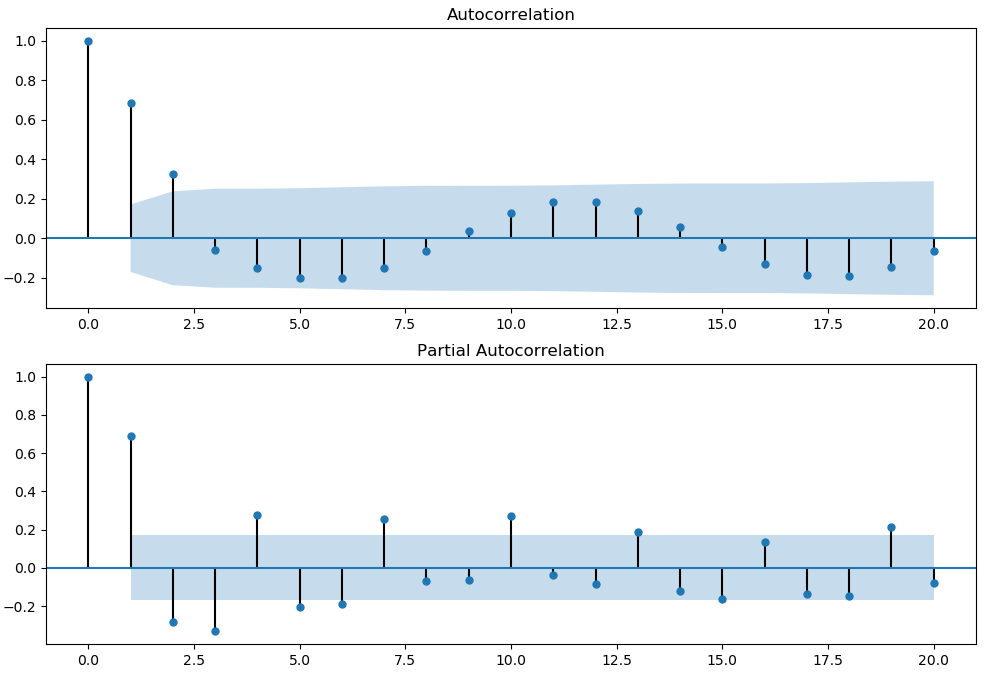
\includegraphics[width=7cm]{./figures/res1.png}
%\caption{fig1}
}
\quad
\subfigure[]{
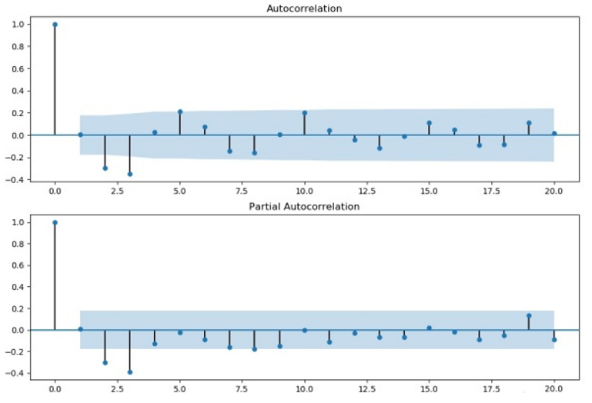
\includegraphics[width=7cm]{./figures/res2.png}
}
\caption{ADF and PADF of trend and residual}
\end{figure}
According to the ADF and PADF result of the trend and residual, we can roughly estimate that :
\begin{enumerate}[(1)]
\item Trend sequence ACF has 3 order tailings, PACF has 2 order tailings, so we can choose $p = 2, q = 3$.
\item Residual sequence ACF has 4 order tailing, PACF has 4 order tailing, so we can choose $p = 4, q = 4$.
\end{enumerate}
When choosing parameters, we need to balance prediction error with model complexity. We can determine the order of the model based on the information criterion function method. Here we introduce a Judging criteria called AIC raised by Akaike in 1971 \cite{9}.
\begin{equation} AIC = -2ln(L) + 2K\end{equation}
If the model's error follows an independent normal distribution, then
\begin{equation} AIC = 2K + nln(\frac{SSR}{n})\end{equation}
Where K is the number of parameter, n is the number of sample and SSR is SUM SQAURE OF RESIDUE. After the test, for trend, $p = 0$, $q = 1$ and for residual $p = 2$, $q =1$.\\
By calculation, we pick the location that is circled by red and use their data to train our model and predict the temperature from 2017.4 to 2019.12. The results are as following , blue is the true value and orange is the predict value.
\textbf{}
\begin{figure}[h]
\centering
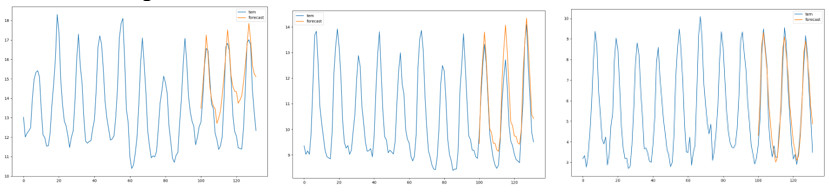
\includegraphics[width=12.5cm]{./figures/new.png}
\caption{Predict result on test set}
\end{figure}
Now we can conclude that the prediction model is reasonable.

\subsubsection{Results}
Base on the prediction model show in 4.2.4, the heatmap of the seawater in different months and different years is shown below. We set the land to zero Celsius in order to distinguish seawater and land easily. When the color of one region looks dark, it means the temperature of seawater in this region is high.

According to the result, there is a noticeable change among seasons, which confirms the validity of our model from the side. In this model, the temperature of the area which is below the Britain in spring (April) and Winter (January) is becoming higher and higher in the next 50 years. At the same time, the temperature of the region close to Greenland and close to the Arctic Ocean is growing higher too. We think the increasement of the temperature is because of global warning which cause the large-scale melt of glacier, indirectly lead to the raise in the north area.

\textbf{}
\begin{figure}[h]
\centering
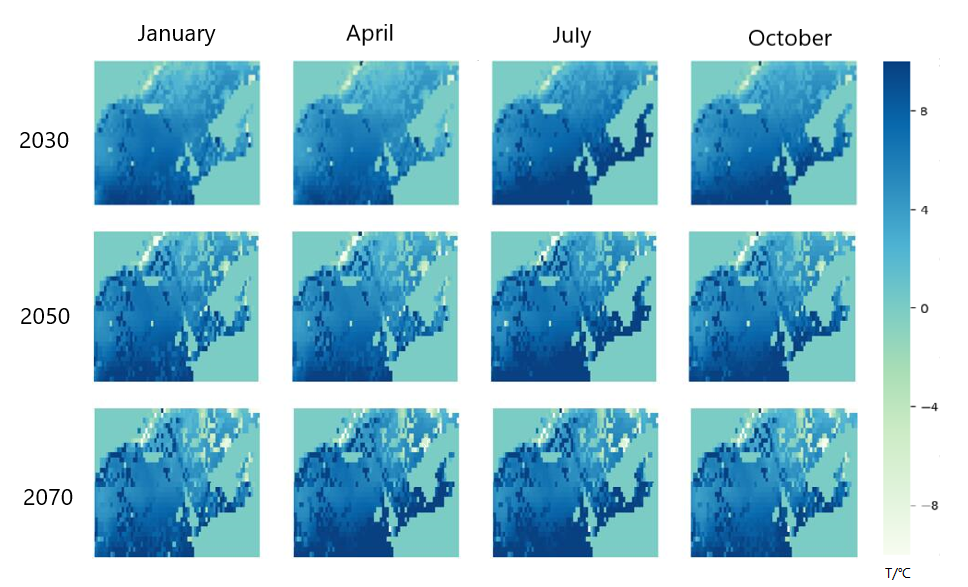
\includegraphics[width=11.5cm]{./figures/f.png}
\caption{Predict result}
\end{figure}\\

%dellete
%For every year, exits an position where it’s fish catches or the fish catches of the place around it is much more higher than other place. We called it the “best position”.
%\item	We only show the affection of mackerel in this chapter for limited space.
%\item In order to represent the temperature change among seasons, we choose January to represent Winter, April to represent Spring, July to represent Autumn and October to represent Autumn. 
\subsection{Time for Warning}
\subsubsection{Introduction}
The growth and development of fish require a suitable temperature and they are sensitive to the change of temperature. Extra expense will be paid by Scotland-based fishing companies because of the longer distance (the cost of fuel) which will make a side effect on fishery (small fishing companies especially).  In this character we will use means shift clustering algorithm to find out the best position to fish and find out its’ character on temperature. Therefore we can predict the gather point or distribution (roughly) of fish according to the future temperature of ocean we already got in last chapter.
\subsubsection{Clustering Process}
Clustering is a machine learning technique that involves grouping data points. Given a set of position points, we can use a clustering algorithm to classify each point into a particular group. \\
(1) Kernel Density Estimation\\
Given $n$ data point, $x_{i}\in R^d$ where $d$ is dimension (latitude, longitude, SPABUN), parameter $h$ is the bandwidth of kernel function $K$. Then the KDE of the dataset is:
\begin{equation} f(x) = \frac{1}{nh^d}\sum_{i=1}^n K(x)\end{equation}
where $K(x)=c_{k,d} k(‖x‖^2)$ ,$ c_{k,d}$ is normalization constant which make the integral of $K(x)$ is 1. Here we choose Radially Symmetric Kernel as our kernel function.
\begin{equation} K(x)=K(\frac{x-x_{i}}{h})\end{equation}
(2) Mean Shift
The basic goal of mean shift is to move the sample points in the direction that  local density is increases. The mean moving vector refers to the direction of local density that increase fastest, so this vector point to the gradient direction of the data set density. The gradient of $f(x)$ is:

\begin{equation}\nabla f(x)=\frac{2c_{k,d}}{nh^5}[\sum_{i=1}^n g(||\frac{x-x_{i}}{h}||^2)]
[\frac{
\sum_{i=1}^n x_{i} g (||\frac{x-x_{i}}{h}||^2)}
{\sum_{i=1}^n g (||\frac{x-x_{i}}{h}||^2)}-x]
\end{equation}
Where $g(s)=-k'(s)$ , so the gradient direction $m_{h} (x)$ is:
\begin{equation}
m_{h}(x)=\frac
{\sum_{i=1}^n x_{i} g (||\frac{x-x_{i}}{h}||^2)}
{\sum_{i=1}^n g (||\frac{x-x_{i}}{h}||^2)}-x
\end{equation}
So at every steps of Mean-shift clustering algorithm is:\\
	(1) Calculate $m_{h} (x)$  of every sample
	(2) $x_{i}=x_{i}+m_{h} (x_{i})$
	(3) Repeat (1) (2), until the sample point is convergent
	(4) The points which converge into the same point are considered they belong to a same cluster

\subsubsection{Temperature of Cluster Center}
In order to get the overall geography trend of the clustering centers, we decide to choose the period from 2009 to 2017 and calculate their clustering point relatively base on the data from ICES (International Association for the Physical Science of the Ocean)\\
Then we plot them in the picture below.
\textbf{}
\begin{figure}[h]
\centering
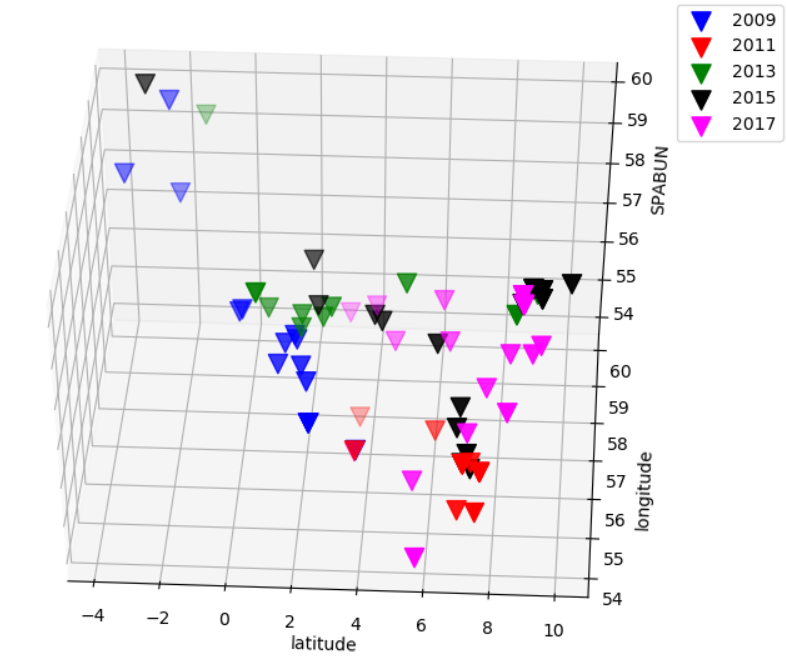
\includegraphics[width=7.5cm]{./figures/cl.png}
\caption{Clustering center distribution}
\end{figure}

From the result we can see that the position tendency of “best points” are leaving England, moving to the south-east. The average temperature of these cluster of each years is:

\textbf{}
\begin{center}
\begin{tabular}{|c|c|}
\hline
\rowcolor{lightgray} \makebox[0.4\textwidth][c] {Year}& \makebox[0.4\textwidth][c] {Average Temperature(℃)} \\ \hline
2009    &14.16	\\ \hline 
2011    &14.94	\\ \hline 
2013    &14.28	\\ \hline 
2015    &13.63	\\ \hline 
2017    &14.02	\\ \hline 
\end{tabular}
\end{center}
We define the Average Temperature(℃) as $T_{b}$. Naturally, we can use liner regression to simulate the change of the average temperature of "best points". 
\begin{equation} T_{b} = \theta x + b + \varepsilon \end{equation}
The result of liner regression is $\theta=0.0815$ , $b=14.61$ and $\varepsilon$ is white noise subject to normal distribution.

\subsubsection{Predict Model and Result}
To determine a region is "best point" or not, we introduce a  criterion $S$. We divided the sea into two kinds: region that all of its neighbor region is sea, called $R_{s}$ and region that some of its neighbor region is land, called  $R_{l}$. Then the criterion for each kind of sea is:
\begin {equation}S = \frac{\begin{matrix} \sum_{j=-1}^1\end{matrix} \begin{matrix} \sum_{i=-1}^1 \end{matrix}
T_{c,ij}(r(lo+i, la+j))}
{9}\end{equation}

Where $T_{c,ij}(r(lo,la))$ is score function:
\begin{equation}
T_{c,ij}=
\begin{cases}
0 \text{\quad if r is $R_{l}$} \\
\frac{\sqrt{2}}{|r(lo,la)-T_{b}|} \text{\quad i=j}\\
\frac{1}{|r(lo,la)-T_{b}|} \text{else}
\end{cases}
\end{equation}
And $r(lo,la)$ is the temperature of a region where its longitude is $lo$ and its latitude is $la$. So for a particular year, in order to find the position of "best point", 
First is calculate $S$ for every grid of the map. Then choose those who S is larger than our threshold. Here we test a group of years from 2020 to 2045, in steps of 2 and choose 5 as our threshold.
\textbf{}
\begin{figure}[h]
\centering
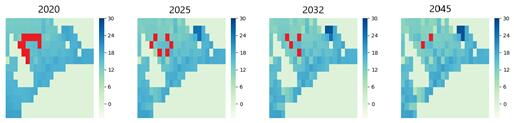
\includegraphics[width=10.5cm]{./figures/best.png}
\caption{best point distribution in the future}
\end{figure}
The red grid represent that this place is probably a “best point” and the pink grid represent that this place has fewer possibilities to be a “best point”. Considering small fishery companies is lack of resource (money, facilities, government permission) to sail far, the places are “best point” but too far away from England is not shown on the picture.
According to the prediction and compare with the location that they fishing now where is shown in Appendix 1, we can preliminary conclude that:\\
(1)	In worst case, the fish in the location that they current operate will keep decline after 2025 and it may cost too much to go to the new “best point” fishing.\\
(2)	In best case, the fish in the location that they current operate will slowly decline after 2020 but after 2045, the new “best point” is too far away.

\section{Strategy of Fishing Companies}
We collect several fisheries in Scotland according to the longitude and latitude on Google Map, combined with the prediction of mackerel's migration before, we can get following figure.
\textbf{}
\begin{figure}[h]
\centering
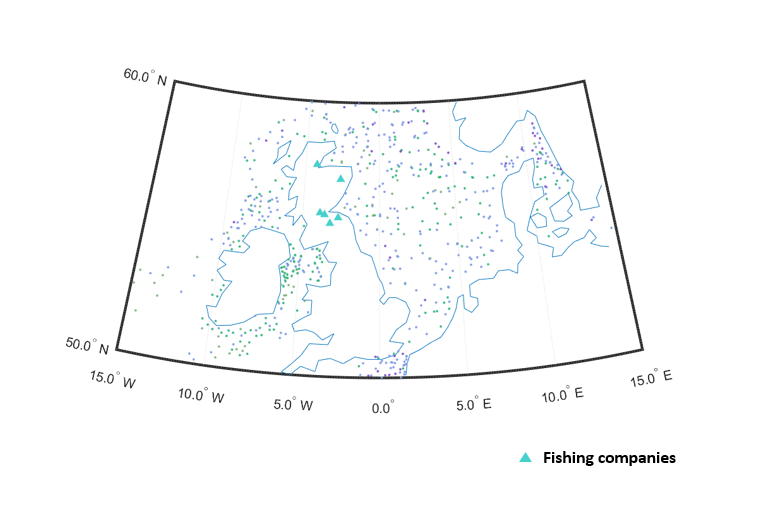
\includegraphics[width=12.5cm]{./figures/fishery.png}
\caption{Fisheries in Scotland \& distribution of mackerel}
\end{figure}\\
Small fishing companies should be aware of migration of herring and mackerel. However, to make reasonable decisions, a reasonable assessment system is needed.
Firstly, we list 4 strategies according to given information as follows:
\begin{itemize}
\item Relocate the whole company
\item Establish a branch company in Northern cities
\item Employ lightweight fishing vessels which are able to work without land supplies
\item Remain the same
\end{itemize} 
\subsection{Comparison between 2 Relocating Stretagies}
Next we analyze the impact of each action.
Relocation means moving the whole company to the north. We find main fisheries in Scotland distribute along the coastline in 2020, consequently we choose the center of these companies as \textbf{the initial location}, the nearest coastline of fish clustering as \textbf{the target location}. Assume that the company move in accordance with herring and mackerel, the effective fishing radius is 10 km. 
Consider the convenience of transportation, all the locations are set in big cities.
The initial location is around Glasgow and the new address is around Inverness.\\

In comparison, if we establish a branch company instead, both two companies will have economic income. However, due to the split of the funds and fishing facilities, the fishing radius decreases to 5 km for each.
The figures are as follows.
\begin{figure}[htbp]
\centering
\subfigure[Relocation]{
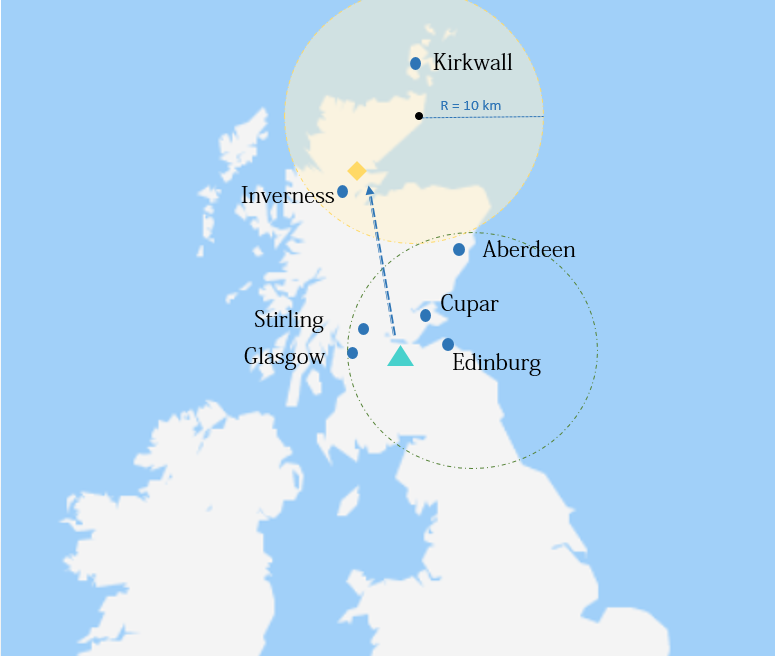
\includegraphics[width=5.5cm]{./figures/s1.png}
%\caption{fig1}
}
\quad
\subfigure[Branch company]{
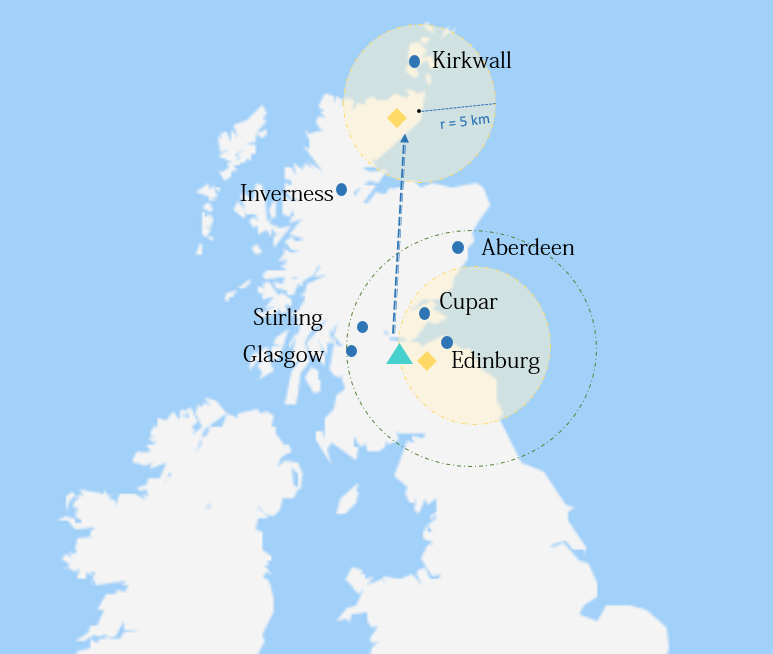
\includegraphics[width=5.5cm]{./figures/s2.png}
}
\caption{Comparison of strategies 1\&2}
\end{figure}

\subsection{Applying lightweight fishing vessels}
The advantage of small vessels lies in its flexibility. We assume a company introduce 3 small vessels which can reach 12 nautical miles(21.6 km) away from coastline . Following figure illustrates the situation.
\textbf{}
\begin{figure}[h]
\centering
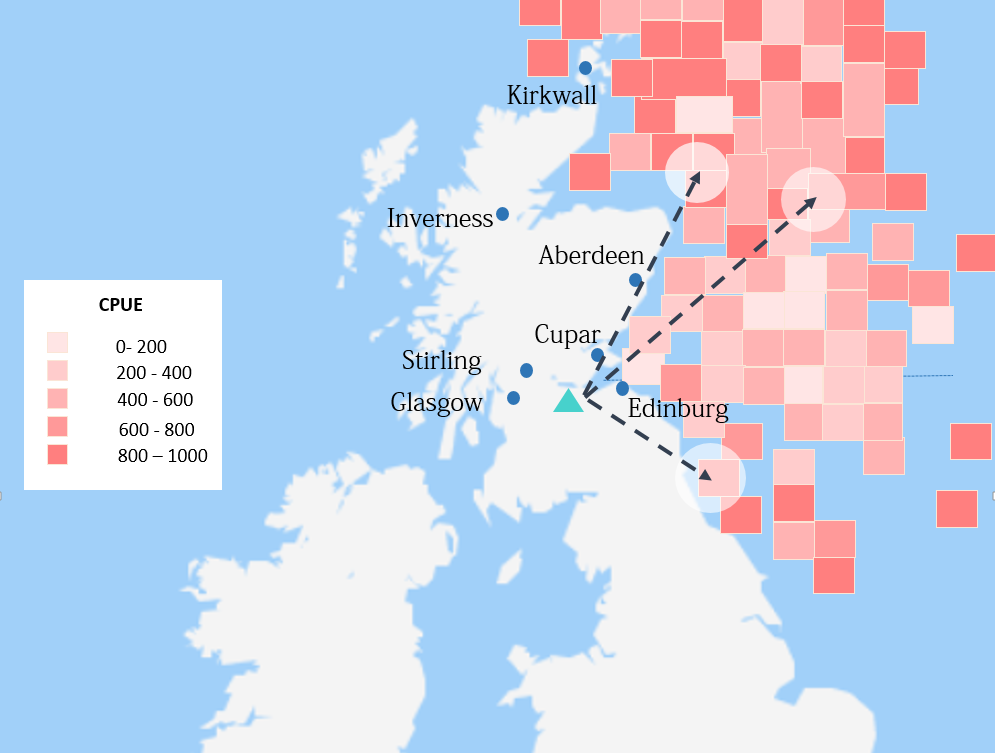
\includegraphics[width=8.5cm]{./figures/s3.png}
\caption{Small vessels applied}
\end{figure}\\

\subsection{Assessment System with TOPSIS}
\textbf{(1) Factors involved}\\
 \hspace*{2em} We use Technique for Order Preference by Similarity to an Ideal Solution (TOPSIS) to build an assessment system.
We introduce 4 separate factors: Funds($F$), Catch Per Unit Effort (CPUE), Maintenance Cost ($M$), Transportation Fee ($T$). 

\begin{itemize}
\item  The index Catch Per Unit Effort (CPUE) is used for measuring the richness of species in a fixed area. The CPUE in the year $y$ can be represented as $CPUE_{y}$
\begin{equation} CPUE_{y} = \frac{C_{y}}{E_{y}}\end{equation}
$C_{y}$ is the total catch yield of the year $y$, $E_{y}$ is the quantity of effort in the year $y$.
Assuming that the fishing area contains $n$ parts of different $CPUE$. The average CPUE of an operation 
Can be calculated by summing up effective areas.
\begin{equation}\overline{CPUE}=\sum_{j=1}^{n} \frac{s_{j}}{S}*CPUE_{j} \end{equation}
$s_{j}$ is the area of $j_{th}$ part, $S$ is the gross area of fishing area, which is related to the number of fishing vessels. \\
This approach to calculating $CPUE$ is generalized and applied in our following model. 
\item $F$ represents the expense of establishing a new company, relocation, spent on new facilities. CPUE is used to describe total quantity of fish.\begin{equation}F = F_{base} + F_{add}\end{equation}, here we set $F_{add}$ for 3 strategies is 7,5,3 respectively. Additionally, we assume the cost of a new small vessel and a common fishing boat is 5 unit and 10 unit respectively.\\
\item $M$ is maintenance cost of facilities.
\begin{equation}M = \sum_{k=1}^n * v_{small} + \sum_{k=1}^m * v_{common}\end{equation}
$n$,$m$ is the quantity of new small vessels and common boats respectively, $v_{small}$ and $v_{common}$ represents the value of two vessels.\\
\item T is the expense on the fuel for traveling, which is closely related to the distance between fishing point to the coast and the distance from the company to selling point. $T$ can be measured by calculating the gross length of one operation, here we get data from Google Map.\\
\end{itemize}



%参数计算和统计
%(CPUE用格子所代表的鱼的密度统计, C 是分公司个数,小型渔船个数的函数,M与船只个数/航行距离有关, T与公司选址到交通枢纽,%捕鱼点到海岸线距离成正比 用谷歌地图测量有关)

\begin{table}[htbp]
\begin{center}
\begin{tabular}{|c|c|c|c|c|}
 \hline
 \rowcolor{lightgray}\makebox[0.1\textwidth][c]{Strategy}& \makebox[0.2\textwidth][c]{Distance/55.4km}
& \makebox[0.2\textwidth][c]{Maintenance} & \makebox[0.2\textwidth][c]{Funds}
& \makebox[0.2\textwidth][c]{CPUE/$10^3$} \\ \hline
1 & 23.12 & 17 &  9.41& 7.25\\[3pt]   \hline
2 & 18.48 & 15 &  9.55& 10\\[3pt]   \hline
3 & 12.61 & 13 &  15.23& 8\\[3pt]   \hline
4 & 12.61 & 10 &  10&    6.3\\[3pt]   \hline
\end{tabular}\\
\end{center}
\caption{Factors Involved}
\end{table}
Strategy 1, 2, 3, 4 stands for relocating to the north, establishing a branch company in the north, applying lightweight fishing wessels and remaining the same respectively.\\

\textbf{(2)Weight of Each Factor}\\
 \hspace*{2em} Using Analytic Hierarchy Process (AHP), we set comparison matrix 
$$A = 
\begin{bmatrix}
1 & 1 & \frac{1}{2} & \frac{1}{2}\\
1 &1 &1& \frac{1}{2}  \\
 \frac{1}{2} & 1 & 1 & \frac{1}{4}  \\
 2 & 2 & 4 & 1\\
\end{bmatrix}$$
 \hspace*{2em} Check value $CR = \frac{CI}{RI} = 0.02 < 0.1$, thus the matrix is reasonable.\\
 \hspace*{2em} Weight : $W = [0.224, 0.192, 0.137, 0.447]$.

\textbf{(3) Assessment results}\\
 \hspace*{2em} Initial data matrix $X$
$$
X = 
\begin{bmatrix}
23.12 & 17 &  9.41& 7.25\\
18.48 & 15 &  9.55& 10\\
12.61 & 13 &  15.23& 8\\
12.61 & 10 &  10&    6.3\\
\end{bmatrix}
$$
 \hspace*{2em} According to  $z_{ij}=\frac{x_{ij}}{\sqrt{\sum_{i=1}^{n}x_{ij}^2}}$, we get standardized matrix $Z$ 
$$
Z = 
\begin{bmatrix}
 0.328 & 0.381 &0.556 & 0.452  \\
 0.411 & 0.432 &0.548 & 0.624   \\
 0.602 & 0.498 & 0.343 & 0.500  \\
 0.602 & 0.648 & 0.523 & 0.394 \\
\end{bmatrix}
$$
 \hspace*{2em} Define:\\ 
 \hspace*{2em} \textbf{the Maximun Value}\\
 \hspace*{2em}  $Z^{+}=(Z^{+}_{1}, Z^{+}_{2},...,Z^{+}_{m}) =(max\{z_{11},z_{21},...z_{n1}\},max\{x_{12},z_{22},...,z_{42}\},..,max\{z_{14},z_{24},...,z_{44}\}) $
 \hspace*{2em} \textbf{the Minimum Value} \\
 \hspace*{2em} $Z^{-}=(Z^{-}_{1}, Z^{-}_{2},...,Z^{-}_{4}) =(min\{z_{11},z_{21},...z_{41}\},min\{x_{12},z_{22},...,z_{42}\},..,min\{z_{14},z_{24},...,z_{44}\}) $
 \hspace*{2em}  The distance between $i_{th}$ (i=1,2,3,4) strategy and $Z^{+}$ is:
\begin{equation}
L^{+}_{i} = \sqrt{\sum_{j=1}^{4}(Z^{+}_{j}-z_{ij})^2}  \quad
L^{-}_{i} = \sqrt{\sum_{j=1}^{4}(Z^{-}_{j}-z_{ij})^2}
\end{equation}
 \hspace*{2em} Score of the $i_{th}$ (i=1,2,3,4) is represented as: 
\begin{equation}
S_{i}=\frac{L^{-}_{i}}{L^{+}_{i}+L^{-}_{i}}
\end{equation}
 \hspace*{2em} We sort 4 strategies by $S_{i}$,$i \in \{1,2,3,4\}$, the result is shown as follows:
\begin{center}
\begin{tabular}{|c|c|c|c|c|c|c|c|c|}
\hline
\rowcolor{lightgray}{Index}&  \makebox[0.1\textwidth][c]{Distance} & \makebox[0.15\textwidth][c] {Maintenance}& \makebox[0.1\textwidth][c] {Funds}& \makebox[0.1\textwidth][c] {CPUE}&{$D^{+}$}
& {$D^{-}$} & \makebox[0.1\textwidth][c]{$S_{i}$}
& \makebox[0.1\textwidth][c]{\textbf{Rank}} \\ \hline
1 & 0.328 & 0.381 &0.556 & 0.452 & 0.209 & 0.088 & 0.296 & 4\\ \hline 
2 & 0.411 & 0.432 &0.548 & 0.624 & 0.131 & 0.178 & 0.576 & 1\\ \hline 
3 & 0.602 & 0.498 & 0.343 & 0.500 & 0.132 & 0.156 & 0.542 & 3\\ \hline 
4 & 0.602 & 0.648 & 0.523 & 0.394 & 0.155 & 0.187 & 0.546 & 2\\ \hline 
\end{tabular}\\
\end{center}

\textbf{}
\begin{figure}[h]
\centering
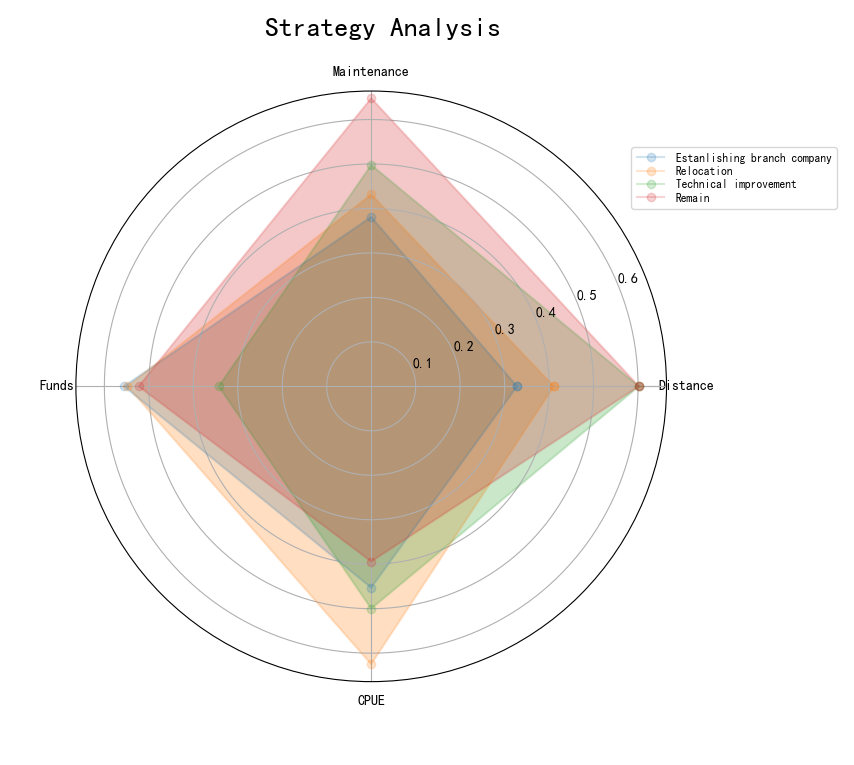
\includegraphics[width=8.5cm]{./figures/cmp.png}
\caption{Strategy Analysis}
\end{figure}
\section{Effect of Territorial waters}
\subsection{Range of territorial waters}
The analysis of 4 responses above proves that Moving to the northern part of the country brings richer marine resources. However, the operation is restricted due to the limited domain of territorial seas. What we want to do is to build a model to analyze the economic loss of practical reason. \\

According to the United Nations Convention on the Law of the Sea (LOSC), maximum of 12 nautical miles from the coastlines (including the coastline of offshore islands) is the territorial seas of a country, where this country is able to utilize surrounding resources. \\
Countries around North Sea and Ireland Sea are Norway, Demark and Ireland. As a result, fishing within their territorial seas is prohibited.

\subsection{Impacts analysis}
Based on the prediction we made, we count the appearance frequency of mackerel during last years, define $L_{y}$ as the quantity of mackerel affected by territorial limits in $y_{th}$ year.
\begin{equation}L_{y} = \frac{c_{y}}{C_{y}}*P_{y}\end{equation}
$s_{y}$ is the  frequency of appearance in available waters in $y_{th}$ year, $S_{y}$ is total appearance of mackerel in Northern Pacific in $y_{th}$ year.

%这里 还需 标注引用!!!!!!!!!!!!!!!!!!!!!!!
Statistics we collected is shown in following chart. Statistics from Fisheries \& Aquaculture Organization(FAO) and
International Council for the Exploration of the Sea (ICES).

\textbf{Production loss due to territorial seas}
\begin{center}
\begin{tabular}{|c|c|c|c|c|c|c|c|c|}
\hline

\rowcolor{lightgray}{Year}&{$C$(/times)} & {$c$(/times)}& {$P$(/t)}& {Hit Rate(${s/S}$)}& {Loss}
& {Percentage}  \\ \hline
1999    &1507	&856	&711634	&0.568   &307414.6   &0.432\\ \hline 
2003	&14499	&5129	&503669	&0.354  &325496.8	 &0.646\\ \hline 
2005	&3720	&1328	&554113	&0.357	&356300.6	&0.643\\ \hline 
2008	&4141	&1328	&442669	&0.321    &300707.1	&0.679\\ \hline 
2010	&13836	&3437	&503669	&0.248	&378552.6	&0.752\\ \hline 
2013	&10181	&2481	&473980	&0.244	&358476.2	&0.756\\ \hline 
2017	&8833	&1824	&581881	&0.206	&461723.5	&0.794\\ \hline 
\end{tabular}\\
\end{center}

\textbf{}
\begin{figure}[h]
\centering
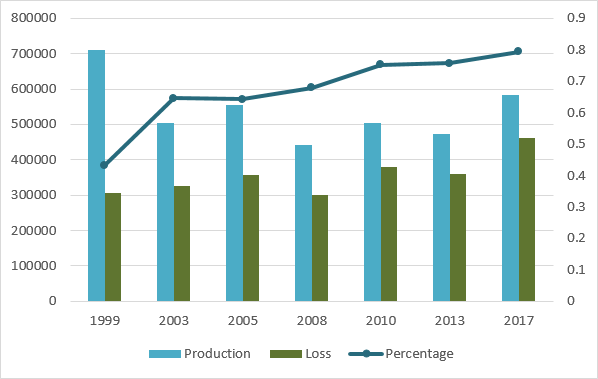
\includegraphics[width=7.5cm]{./figures/ana.png}
\caption{Change curve of the loss}
* Pertentage is used for measuring the diminution casused by territorial problems.
\end{figure}\\

As the chart illustrates, the loss quantity due to territorial seas keeps increasing year by year, which matches the migration of mackerel to the north. Due to the rising sea temperature, habitants of mackerel moves north from 55°N to 60°N. As a result, it is necesssary for small fishing companies around the North Sea to change operatng strategies and push forward innovation.

\section{Model Test}
\subsection{Error Analysis of GAM}
\quad For GAM:
\begin{equation}In DS_{i,(\lambda,\phi)} = a + s1(\lambda_i,\phi_i) + s2(SST_i)+\beta*SSB_i + \varepsilon\end{equation}
The estimated results of parameters are in the Table 7.
\begin{table}[htbp]
\centering
\caption{The Estimated Results of Parameters }
\begin{tabular}{c|cccc}
 \hline
 \rowcolor{lightgray}\makebox[0.15\textwidth][c]{}& \makebox[0.15\textwidth][c]{Estimate}&\makebox[0.15\textwidth][c]{Std. Error}& \makebox[0.15\textwidth][c]{t value}& \makebox[0.15\textwidth][c]{Pr(>|t|)}\\ \hline
 a &13.29251  &  0.16794 & 79.151&0.000124	\\[3pt]
SSB    &0.11987  &  0.03898 &  3.075 & 0.087775\\[3pt]   \hline
\rowcolor{lightgray} \hline
 &edf&  Ref.df&  F & p-value	\\[3pt]  \hline
 $\lambda$ &1&    1&  29.217 & 0.0295	\\[3pt]
$\phi$    &1.933 & 1.995 &26.228 & 0.0320\\[3pt]
$SST$    & 1.000 & 1.000 & 0.264 & 0.6568\\[3pt]   \hline
\end{tabular}\\

\end{table}

$R-sq.(adj) =  0.981$  and deviance explained =$ 99.4\%$.

$R-sq.(adj)$ is close to 1, and indicates that the model fitting effect is excellent.


\subsection{Sensitivity Analysis of Continuous-time Markov Model}

The Regression Square Sum:$S_reg=\Sigma^n_{i=1}(\hat{y_i}-\bar{y})^2$

The Residual Square Sum:$S_res=\Sigma^n_{i=1}(y_i-\hat{y_i})^2$

Where n denote the sample size, m denote the number of countries. The total square sum  can be divided into parts of the regression square sum
(SSR) and the residual square sum (SSE)
\begin{equation}
MSR=SSR/(m-1)
\end{equation}
\begin{equation}
MSE=SSE/(n-m-1)
\end{equation}
\begin{equation}
F=\frac{MSR}{MSE}=\frac{SSR/(m-1)}{SSE/(n-m-1)}
\end{equation}
 We calculated that $F > F_{0.05}(m-1,n-m-1)$.The regression equation is significant under the
significance level $\alpha=0.05$.
\subsection{Temperature prediction}
The threshold is determine subjective, which will influence the number and position of “best point”. So we test the sensitivity by valuation. We change the value of threshold in steps of 0.02 from 5.06 to 4.92.
\textbf{}
\begin{figure}[h]
\centering
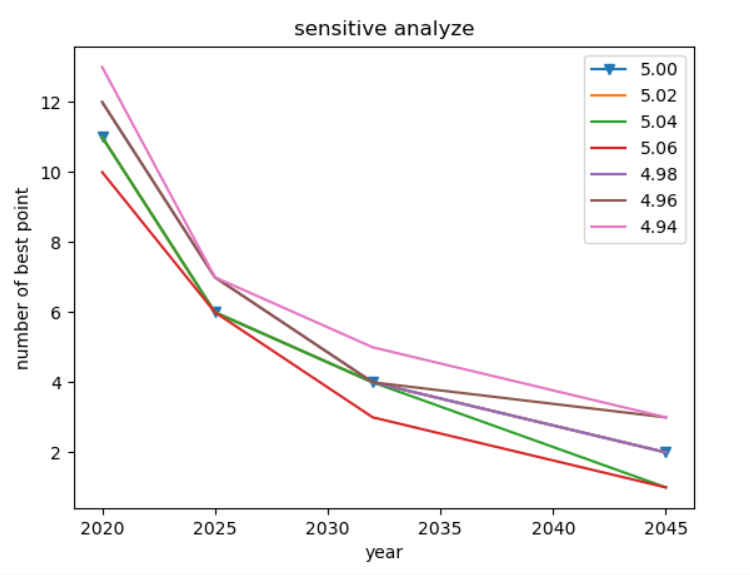
\includegraphics[width=8.5cm]{./figures/sen.png}
\caption{ Sensitive analyze on threshold}
\end{figure}\\
From the graph we can say that the have little affection on the number of best point. As for the position, the biggest change is very small, which can be seen in Appendix 2 for detail. The model is available, the worst case is around 2025, the best case is around 2045.



\section{Strengths and Weaknesses}
\subsection{Strengths}
\begin{itemize}
\item \textbf{Applies widely}\\
The model can be used to predict the future migration of other animals, such as African zebras and birds.
\item \textbf{The model is stable and reliable}\\
Our models are robust while the parameters changes. That is to say, a slight
change of parameter will not cause a significant change of the results.

\item \textbf{Great accuracy}\\
The time series model represents the influence of the historical information of each variable on the situation of the system and entirely describes the dynamic law of the change of temperature.

\item \textbf{Reliable data}\\
Our data comes from the official website such as Fisheries \& Aquaculture Organization(FAO) and
International Council for the Exploration of the Sea (ICES).
\item \textbf{Easy appliance}\\
Do not need to choose the cluster number. Unlike traditional k-means algorithm, mean-shift don’t need to choose how many cluster. TOPSIS provides a direct assessment of strategies. With weight of factors given, the rank is easy to understand.\\
\end{itemize}


\subsection{Weaknesses}
\begin{itemize}
\item \textbf{Factors neglected}\\
Temperature predict model didn’t consider the affect from salt. In the strategy assessment system, we only consider several primary factors impacting strategy choice.
\item \textbf{Rough measurement}\\
The measurement of distance on the sea is rough, the statistics about the distribution of mackerel is not complete.
\item \textbf{Complex data}\\
The data of some parameters is forecast data because we do not have real practical
experience.
\end{itemize}
\clearpage

\section{A Letter}
\textbf{MEMORANDUM}~\\
\textbf{TO: Hook Line and Sinker}\\
\textbf{FROM:Team \#2010755}\\

With the increase of ocean temperature, marckerel and herring will migrate to higher latitudes, searching for a suitable place to settle down since the metabolism of fish accelerates once the surrounding temperature rises. That is the reason why they require more oxygen and food yet higher temperature reduces oxygen solubility of seawater, which leads to the death of fish. At the same time, some fish can’t spawning when the temperature is higher than a threshold. Both Scottish herring and mackerel play an important role in the Scottish fishing industry. But unfortunately, according to our research, they are trying to escape from England.\\

\textbf{Where do they want to go}\\
Based on former data and consider the influence of temperature, our team build a model to predict the distribution of herring and mackerel in the next 50 years. The result shows that during the next 50 years, herring will migrate to Gulf of Bothnia and mackerel will migrate to Norwegian Sea --- both of them will be more than 900km away from Scotland at that time.\\

\textbf{Suggestions to small fishery company}\\
In order to achieve higher profitability or just to maintain the profit, companies should take actions such as relocating the whole company, establishing a branch company in the Northern cities or employing lightweight fishing vessels. All of these methods work to some extent. With various factors taken into account, building a new branch company in the Northern is the best choice by which companies can get closer to fish resources. Additionally, it costs less compared with other solutions such as relocating the whole company.\\

\textbf{Suggestions to a normal fisherman}\\
With the depletion of fishery resources, there are two ways to for fishermen to increase or maintain their income. One of them is to change the traditional ways to catch fish. Fishermen are able to "farming" in the sea, cultivating economic fish in shallow waters. The other one is to develop recreational fishing for tourists. Picking tourists to the beautiful seaside and teaching them how to fish during the fishing off-season must be a great pleasure. At the same time, it brings enormous economic benefits as well.\\

\textbf{Thank you for your consultation!}\\

\textbf{ Best Wishes, Team \#2010755}\\


\begin{thebibliography}{99}
\bibitem{1} Olafsdottir, A. H., Utne, K. R., Jacobsen, J. A., Jansen, T., Óskarsson, G. J., Nøttestad, L., ... \& Slotte, A. (2019). Geographical expansion of Northeast Atlantic mackerel (Scomber scombrus) in the Nordic Seas from 2007 to 2016 was primarily driven by stock size and constrained by low temperatures. Deep Sea Research Part II: Topical Studies in Oceanography, 159, 152-168.
\bibitem{2}  Wu shengnan, Chen xinjun, \& liu zhonan. (2019). Prediction model of Japanese mackerel resource abundance in the northwest Pacific based on GAM. Acta oceanologica sinica, 41(8), 36-42.
\bibitem{3}\url{http://ecosystemdata.ices.dk/Map/index.aspx?Action=AddLayer&TAXA=6799&YEAR=2017&Grid=-1&Color=random&Type=Count}
\bibitem{4} Nøttestad, L., Anthonypillai, V., Tangen, Ø., Høines, A., Utne, K. R., Oskarsson, G. J., ... \& Jansen, T. (2016). Cruise report from the International Ecosystem Summer Survey in the Nordic Seas (IESSNS) with M/V M. Ytterstad’, M/V ‘Vendla’, M/V ‘Tróndur ı Gøtu’, M/V ‘Finnur Frıði’and R/V ‘Arni Friðriksson, 1-31.
\bibitem{5} Zhang yunquan, zhu yaohui, li cunlu, feng renjie, \& ma lu. (2015). Implementation of generalized additive model in R software. China health statistics, 32(6), 1073-1075.
\bibitem{6}Li dewei, zhang long, wang Yang, \& zhu wenbin. (2015). Analysis of the relationship between CPUE and environmental factors in Argentine sliders based on GAM. Fisheries modernization, (2015 04), 56-61.
\bibitem{7}XiaoXin Han(2009). Research on the Contribution Rates of Three Industries in
China Based on Markov Chain. Cooperative Economy \& Science (15), 24-25.
\bibitem{8}Chang, X., Gao, M., Wang, Y., \& Hou, X. (2012). Seasonal autoregressive integrated moving average model for precipitation time series. Journal of Mathematics \& Statistics, 8(4).
\bibitem{9}
Akaike H. (1987) Factor Analysis and AIC. In: Parzen E., Tanabe K., Kitagawa G. (eds) Selected Papers of Hirotugu Akaike. Springer Series in Statistics (Perspectives in Statistics). Springer, New York, NY
\end{thebibliography}

\begin{appendices}

\section{First appendix}

Here are simulation programmes we used in our model as follow.\\

\textbf{Part 1}

Limited by space, only the code for calculating the distribution of mackerel is listed.

\textbf{\textcolor[rgb]{0.98,0.00,0.00}{Generalized additive model(GAM):}}
\lstinputlisting[language=R]{./code/GAM.R}
\textbf{\textcolor[rgb]{0.98,0.00,0.00}{Optimization of GAM}}
\lstinputlisting[language=R]{./code/GAM_improved.R}
\textbf{\textcolor[rgb]{0.98,0.00,0.00}{fish.txt}}
\lstinputlisting[language=R]{./code/fish.txt}
\textbf{\textcolor[rgb]{0.98,0.00,0.00}{ Markov Model}}
%\lstinputlisting[language=Python]{./code/ma.py}
\textbf{\textcolor[rgb]{0.98,0.00,0.00}{The following data are the 30 state transition matrices calculated.}}
\lstinputlisting[language=Python]{./code/ma_result.txt}
\textbf{Appendix}
\begin{figure}[h]
\centering
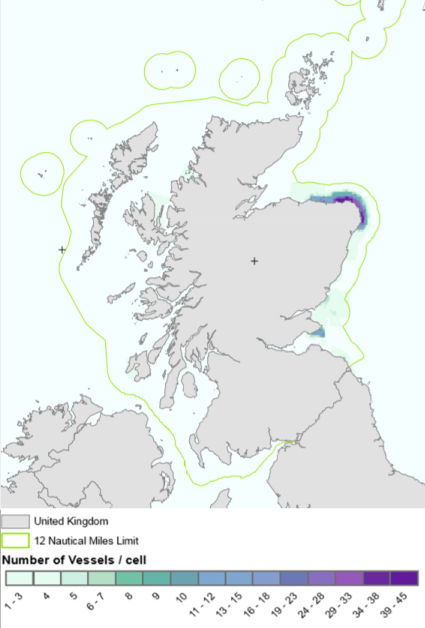
\includegraphics[width=6.5cm]{./figures/map.png}
\caption{ Number of vessels in Scotland}
\end{figure}
\end{appendices}
\textbf{Appendix 1}
\begin{figure}[htbp]
\centering
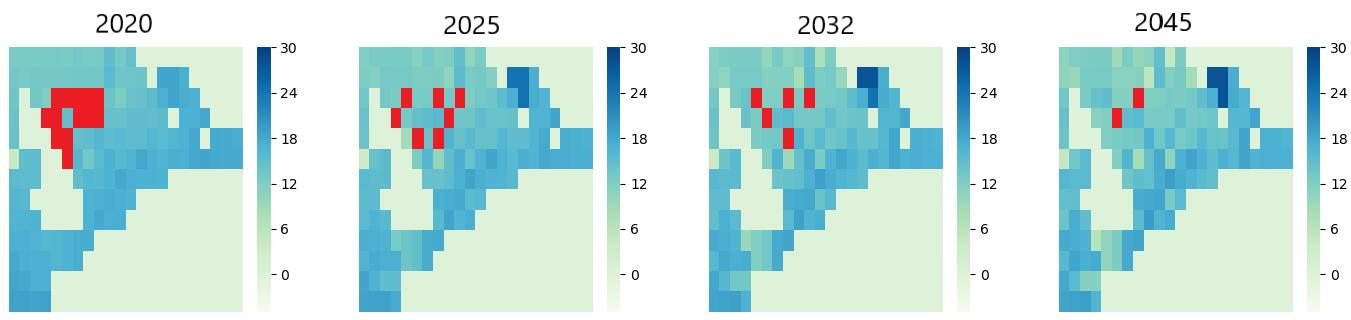
\includegraphics[width=10.5cm]{./figures/appendix_1.png}
\caption{Fisheries in Scotland \& distribution of mackerel}
\end{figure}\\
\end{document}

%%
%% This work consists of these files mcmthesis.dtx,
%%                                   figures/ and
%%                                   code/,
%% and the derived files             mcmthesis.cls,
%%                                   mcmthesis-demo.tex,
%%                                   README,
%%                                   LICENSE,
%%                                   mcmthesis.pdf and
%%                                   mcmthesis-demo.pdf.
%%
%% End of file `mcmthesis-demo.tex'.

\end




